% !TeX root = surprises.tex

\chapter{Der Zusammenfallenden Zirkel}\label{c.collapse}

%%%%%%%%%%%%%%%%%%%%%%%%%%%%%%%%%%%%%%%%%%%%%%%%%%%%%%%%%%%%%%%

Ein moderner Kompass ist ein \emph{fester Kompass}: der Abstand zwischen den beiden Schenkeln kann festgelegt werden, so dass es möglich ist, ein Liniensegment oder einen Kreis von einer Position zu einer anderen zu kopieren (Abb.~\ref{fig.fixed-compass}). Euklid verwendete einen \emph{zusammenfallenden Zirkel}\index{Zusammenfallender Zirkel}, wenn ein fester Abstand nicht eingehalten werden kann (Abb.~\ref{fig.collapsing-compass}). Lehrer verwenden häufig einen Zirkel, der aus einem an einer Schnur befestigten Marker besteht, mit dem man einen Kreis auf einer Tafel konstruiert. Es ist unmöglich, eine feste Länge beizubehalten, wenn der Zirkel von der Tafel entfernt wird. 

\begin{figure}[htb]
\begin{minipage}{.45\textwidth}
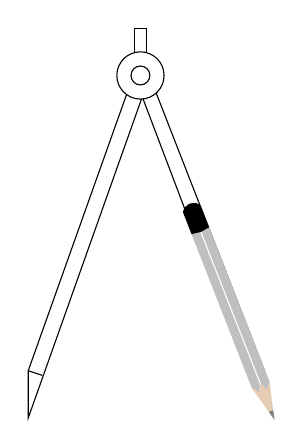
\begin{tikzpicture}
\begin{scope}[rotate=0,transform shape,scale=3]
\draw (2.95,3.7) rectangle (3,3.95);
\draw (2.92,3.68) -- (2.5,2.5) -- (2.5,2.3) -- (2.99,3.68);
\draw (3.5,2.5) -- (3.43,2.48) -- (2.975,3.68);
\draw (3.04,3.68) -- (3.5,2.5);
\draw (2.5,2.5) -- (2.56,2.48);
\draw[fill=white] (2.975,3.75) circle (0.1cm);
\draw (2.975,3.75) circle (0.04cm);
\end{scope}
\begin{scope}[xshift=10.34cm,yshift=7.28cm,rotate=21.4,scale=.6]          
\fill[gray!50] (0,4) -- (0.4,4) -- (0.4,0) --
               (0.3,-0.15) -- (0.2,0) -- (0.1,-0.14) --
               (0,0) -- cycle;
\draw[color=white] (0.2,4) -- (0.2,0);
\fill[black] (0,3.5) -- (0.2,3.47) -- (0.4,3.5) --
             (0.4,4) arc(30:150:0.23cm);
\fill[brown!40] (0,0) -- (0.2,-0.8)
    node[coordinate,pos=0.75](a){} -- 
    (0.4,0)node[coordinate,pos=0.25](b){} -- 
    (0.3,-0.15) -- (0.2,0) -- (0.1,-0.14) -- cycle;
\fill[gray] (a) -- (0.2,-0.8) -- (b) -- cycle;
\end{scope}
\end{tikzpicture}
\caption{Ein fester Kompass. Ein Schenkel hat eine Nadel, die im Mittelpunkt des Kreises platziert wird. Am anderen Schenkel ist ein Bleistift befestigt, mit dem der Kreis gezeichnet wird. Die Schenkel sind durch ein festes Scharnier verbunden, so dass der Abstand zwischen den Schenkeln (der Radius des Kreises) auch dann beibehalten wird, wenn der Zirkel vom Papier abgehoben wird.}\label{fig.fixed-compass}
\end{minipage}
\hfill
\begin{minipage}{.45\textwidth}
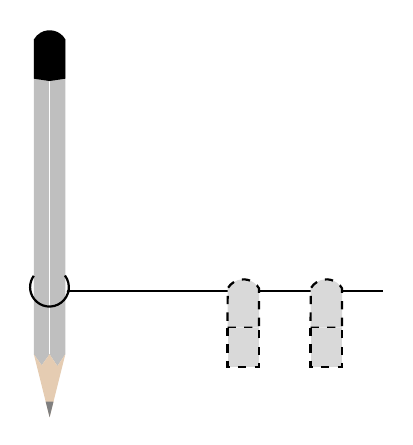
\begin{tikzpicture}[rotate=0,scale=1]          
\fill[gray!50] (0,4) -- (0.4,4) -- (0.4,0) --
               (0.3,-0.15) -- (0.2,0) -- (0.1,-0.14) --
               (0,0) -- cycle;
\draw[color=white] (0.2,4) -- (0.2,0);
\fill[black] (0,3.5) -- (0.2,3.47) -- (0.4,3.5) --
             (0.4,4) arc(30:150:0.23cm);
\fill[brown!40] (0,0) -- (0.2,-0.8)
    node[coordinate,pos=0.75](a){} -- 
    (0.4,0) node[coordinate,pos=0.25](b){} -- 
    (0.3,-0.15) -- (0.2,0) -- (0.1,-0.14) -- cycle;
\fill[gray] (a) -- (0.2,-0.8) -- (b) -- cycle;

\draw[thick] (0.395,1) arc (37:-216:7pt);
\coordinate (knot) at (0.44,.8);
\draw[thick] (knot) -- +(4,0);
\fill (knot) circle (.7pt);

\begin{scope}[xshift=100pt,yshift=-90pt]
\draw[dashed,thick,fill=white!70!gray] (0,3.5) -- (0.4,3.5) -- 
      (0.4,4) arc(30:150:0.23cm) -- cycle;
\draw[dashed,thick,fill=white!70!gray] (0,3.5) -- ++(0,-.5) -- ++(.4,0) -- ++(0,.5);
\end{scope}

\begin{scope}[xshift=70pt,yshift=-90pt]
\draw[dashed,thick,fill=white!70!gray] (0,3.5) -- (0.4,3.5) -- 
      (0.4,4) arc(30:150:0.23cm) -- cycle;
\draw[dashed,thick,fill=white!70!gray] (0,3.5) -- ++(0,-.5) -- ++(.4,0) -- ++(0,.5);
\end{scope}
\end{tikzpicture}
\caption{Ein kollabierender Kompass. Der Benutzer hält ein Stück Schnur in der Mitte des Kreises. Das andere Ende der Schnur ist an einen Bleistift gebunden und wird zum Zeichnen des Kreises verwendet. Wenn der Zirkel vom Papier abgehoben wird, können die Finger (gestrichelt) leicht in eine neue Position rutschen.}\label{fig.collapsing-compass}
\end{minipage}
\end{figure}

This chapter begins with a discussion of the relevance of studying construction with a straightedge and compass (Sect.~\ref{s.relevance}).
Section~\ref{s.collapse} compares the two types of compasses in the most elementary construction: a perpendicular bisector. Section~\ref{s.collapse-copy} presents Euclid's method of copying a line segment using a collapsing compass. This proves that any construction that can be done using a fixed compass can be performed using a collapsing compass. Section~\ref{s.collapse-copy-incorrect} shows a proof of this theorem which seems to be correct, but does not work for all configurations of lines and points. To emphasize that one must not trust diagrams, Sect.~\ref{s.collapse-isoceles} presents a famous alleged proof that all triangles are isoceles; the proof appears to be correct but it is not because the proof is based on an incorrect diagram.

\section{Konstruktion mit Lineal und Zirkel}\label{s.relevance}

Die Konstruktion mit Lineal und Zirkel war früher das grundlegende Konzept, das in der euklidischen Geometrie gelehrt wurde. In letzter Zeit ist es in den Lehrplänen der Schulen in Ungnade gefallen. Es ist sicherlich richtig, dass das Thema, wenn überhaupt, nur wenig praktischen Nutzen hat. Wie wir in den Abschnitten ~\ref{s.neusis}, \ref{s.neusis-doubling}, \ref{s.q}, \ref{s.square-quad} zeigen, wussten die Griechen, wie man Konstruktionen, die mit Lineal und Zirkel unmöglich sind, mit nur geringfügig fortschrittlicheren Werkzeugen durchführen kann. Heute können Computer mit Hilfe numerischer Methoden Konstruktionen mit beliebiger Genauigkeit durchführen.

Dennoch glaube ich, dass es Vorteile hat, Konstruktionen zu studieren:
\begin{itemize}
\item Es macht mehr Spaß und ist eine größere Herausforderung, Geometrie durch Konstruktionen zu lernen, als einfach nur Theoreme und Beweise zu lesen.
\item Bedeutende Durchbrüche in der Mathematik wurden durch Versuche erzielt, Konstruktionen zu finden. In Kapitel~\ref{c.heptadecagon} wird eine Konstruktion von Gauß vorgestellt, die zur modernen abstrakten Algebra geführt hat, insbesondere zu der von \'{E}variste Galois entwickelten Theorie.\index{Galois, Evariste@Galois, \'{E}variste}
\item Es ist etwas kontraintuitiv und daher sehr interessant, dass bewiesen werden kann, dass es unmöglich ist, einige geometrische Objekte zu konstruieren.
\item Traurigerweise gibt es viele Menschen, die Jahre ihres Lebens mit dem Versuch verschwenden, unmögliche Konstruktionen durchzuführen. Schülerinnen und Schüler sollten sich der Vergeblichkeit solcher Bemühungen durchaus bewusst sein.
\end{itemize}

\section{Feste Kompasse und zusammenklappbare Kompasse}\label{s.collapse}

In einigen Geometrie-Lehrbüchern wird die Konstruktion einer rechtwinkligen Winkelhalbierenden\index{Kollabierender Zirkel!Konstruktion einer rechtwinkligen Winkelhalbierenden} eines Linienabschnitts dargestellt, indem zwei Kreise konstruiert werden, die an den Enden des Linienabschnitts zentriert sind, so dass die Radien gleich und \emph{größer als die halbe Länge des Abschnitts} sind (Abb.~\ref{f.collapse-perp-bisector-fixed}). Dies ist nur mit einem festen Zirkel möglich, da nach dem Zeichnen des Kreises in der Mitte von $A$ der Abstand zwischen den Schenkeln des Zirkels fest bleiben muss, um den Kreis in der Mitte von $B$ zu zeichnen.

\begin{figure}[t]
\begin{minipage}{.45\textwidth}
\begin{tikzpicture}[scale=0.5]
\coordinate (A) at (0,0);
\coordinate (B) at (4,0);
\vertex{A};
\vertex{B};
\draw (A) node[below left] {$A$} -- (B) node[below right] {$B$};
\draw[name path=larc] (A) ++(-60:3cm) arc (-60:60:3cm);
\draw[name path=rarc] (B) ++(-120:3cm) arc (-120:-240:3cm);
\path [name intersections={of=larc and rarc,by={b,t}}];
\node[above right,xshift=-2pt,yshift=5pt] at (t) {$C$};
\node[below left,xshift=2pt,yshift=-5pt] at (b) {$D$};
\draw ($ (b) ! 1.2 ! (t)$) -- ($ (t) ! 1.2 ! (b)$);
\end{tikzpicture}
\caption{Konstruktion einer Mittelsenkrechten mit einem festen Zirkel}\label{f.collapse-perp-bisector-fixed}
\end{minipage}
\hfill
\begin{minipage}{.45\textwidth}
\begin{tikzpicture}[scale=0.5]
\coordinate (A) at (0,0);
\coordinate (B) at (4,0);
\vertex{A};
\vertex{B};
\draw (A) node[below left] {$A$} -- (B) node[below right] {$B$};
\draw[name path=larc] (A) ++(-80:4cm) arc (-80:80:4cm);
\draw[name path=rarc] (B) ++(-100:4cm) arc (-100:-260:4cm);
\path [name intersections={of=larc and rarc,by={b,t}}];
\node[above right,xshift=-2pt,yshift=3pt] at (t) {$C$};
\node[below left,xshift=2pt,yshift=-3pt] at (b) {$D$};
\draw ($ (b) ! 1.2 ! (t)$) -- ($ (t) ! 1.2 ! (b)$);
\end{tikzpicture}
\caption{Konstruktion einer Mittelsenkrechten mit einem festen oder einem zusammenfallenden Zirkel}\label{f.collapse-perp-bisector-collapse}
\end{minipage}
\end{figure}

Abbildung~\ref{f.collapse-perp-bisector-collapse} zeigt die Konstruktion einer Mittelsenkrechten entweder mit einem festen oder einem zusammenfallenden Zirkel. Es werden zwei Kreise konstruiert: einer mit Mittelpunkt $A$ und Radius $\overline{AB}$ und einer mit Mittelpunkt $B$ und Radius $\overline {BA}$. Dies kann mit einem kollabierenden Zirkel geschehen, weil (offensichtlich) $\overline{AB}=\overline{BA}$ ist, so dass der Zirkel sich nicht die Länge von $\overline{AB}$ merken muss, um einen Kreis mit dem Mittelpunkt $B$ und demselben Radius zu konstruieren.
Der Beweis, dass die in Abb.~\ref{f.collapse-perp-bisector-fixed} konstruierte Linie eine rechtwinklige Winkelhalbierende ist, ist keineswegs elementar, da relativ fortgeschrittene Konzepte wie kongruente Dreiecke verwendet werden müssen. Der Beweis, dass die in Abb.~\ref{f.collapse-perp-bisector-collapse} gezeigte Konstruktion einer rechtwinkligen Winkelhalbierenden korrekt ist, ist jedoch einfach und basiert auf der Tatsache, dass $\triangle ABC$ ein gleichseitiges Dreieck ist. In der Tat ist dies der erste Satz in Euklids \textit{Elemente}.\index{Euklids Elemente@Euklids \textit{Elemente}}
$\overline{AC}=\overline{AB}$, da es sich um Radien desselben Kreises handelt, und in ähnlicher Weise $\overline{BC}=\overline{BA}$. Wir haben: $
\overline{AC}=\overline{AB}=\overline{BA}=\overline{BC}$.

Abbildung~\ref{f.collapse-equilateral-fixed} zeigt, dass das Dreieck bei der Konstruktion mit festem Zirkel ein gleichschenkliges und nicht unbedingt ein gleichseitiges Dreieck ist \index{Kollapsierender Zirkel!Konstruktion eines gleichseitigen Dreiecks} (Abb.~\ref{f.collapse-equilateral-collapse}).

\section{Euklids Konstruktion zum Kopieren eines Linienabschnitts}\label{s.collapse-copy}

Der zweite Satz von Euklids \textit{Elemente}\index{Euklids Elemente@Euklids \textit{Elemente}} beschreibt, wie man ein gegebenes Liniensegment $\overline{AB}$ in ein Segment gleicher Länge kopiert, dessen einer Endpunkt ein gegebener Punkt $C$ ist. Daher bringt ein fester Zirkel keine zusätzlichen Fähigkeiten mit sich und ein kollabierender Zirkel ist ausreichend, obwohl die Konstruktionen mit einem festen Zirkel einfacher sind.

\begin{theorem}
Gegeben ein Liniensegment $\overline{AB}$ und einen Punkt $C$, kann ein Liniensegment $\overline{CC'}$, dessen einer Endpunkt $C$ ist, mit Hilfe eines zusammenfallenden Zirkels konstruiert werden, so dass $\overline{AB}=\overline{CC'}$ (Abb.~\ref{f.collapse-copying-1}).
\end{theorem}

\begin{figure}[t]
\begin{minipage}{.45\textwidth}
\begin{tikzpicture}[scale=0.5]
\coordinate (A) at (0,0);
\coordinate (B) at (4,0);
\vertex{A};
\vertex{B};
\draw (A) node[below left] {$A$} -- (B) node[below right] {$B$};
\draw[name path=larc] (A) ++(-60:3cm) arc (-60:60:3cm);
\draw[name path=rarc] (B) ++(-120:3cm) arc (-120:-240:3cm);
\path [name intersections={of=larc and rarc,by={b,t}}];
\vertex{t};
\vertex{b};
\node[above right,xshift=-2pt,yshift=5pt] at (t) {$C$};
\node[below left,xshift=2pt,yshift=-5pt] at (b) {$D$};
\draw (A) -- (t);
\draw (B) -- (t);
\end{tikzpicture}
\caption{Konstruktion eines isokratischen Dreiecks mit einem festen Zirkel}\label{f.collapse-equilateral-fixed}
\end{minipage}
\hfill
\begin{minipage}{.45\textwidth}
\begin{tikzpicture}[scale=0.5]
\coordinate (A) at (0,0);
\coordinate (B) at (4,0);
\draw (A) node[below left] {$A$} -- (B) node[below right] {$B$};
\vertex{A};
\vertex{B};
\draw[name path=larc] (A) ++(-80:4cm) arc (-80:80:4cm);
\draw[name path=rarc] (B) ++(-100:4cm) arc (-100:-260:4cm);
\path [name intersections={of=larc and rarc,by={b,t}}];
\vertex{t};
\vertex{b};
\node[above right,xshift=-2pt,yshift=3pt] at (t) {$C$};
\node[below left,xshift=2pt,yshift=-3pt] at (b) {$D$};
\draw (A) -- (t);
\draw (B) -- (t);
\end{tikzpicture}
\caption{Konstruktion eines gleichseitigen Dreiecks mit einem zusammenklappbaren Zirkel}\label{f.collapse-equilateral-collapse}
\end{minipage}
\end{figure}

\begin{figure}[b]
\begin{minipage}{.45\textwidth}
\begin{tikzpicture}[scale=0.5]
\coordinate (C) at (0,0);
\coordinate (A) at (3,0);
\draw (A) node[below,xshift=-2pt,yshift=-2pt] {$A$} -- +(40:4) coordinate (B) node[right] {$B$};
\vertex{A};
\vertex{B};
\vertex{C};
\node[below,xshift=2pt,yshift=-2pt] at (C) {$C$};
\draw[thick,dashed] (C) -- +(160:4) coordinate (D) node[below] {$C'$};
\vertex{D};
\end{tikzpicture}
\caption{Kopieren Sie das Liniensegment $\overline{AB}$. Die Ausrichtung von $\overline{CC'}$ ist nicht wichtig.}\label{f.collapse-copying-1}
\end{minipage}
\hfill
\begin{minipage}{.45\textwidth}
\begin{tikzpicture}[scale=0.5]
\coordinate (C) at (0,0);
\coordinate (A) at (3,0);
\draw (A) node[below,xshift=-2pt,yshift=-2pt] {$A$} -- +(40:4) coordinate (B) node[right] {$B$};
\vertex{B};
\node[below,xshift=2pt,yshift=-2pt] at (C) {$C$};
\draw (A) -- (C);
\path[name path=larc] (C) ++(-70:2.5cm) arc (-70:70:2.5cm);
\path[name path=rarc] (A) ++(-110:2.5cm) arc (-110:-250:2.5cm);
\path [name intersections={of=larc and rarc,by={d,D}}];
\node[above] at (D) {$D$};
\draw (A) -- (D);
\draw (C) -- (D);
\end{tikzpicture}
\caption{Kopieren eines Liniensegments mit einem zusammenfallenden Zirkel}\label{f.collapse-copying-2}
\end{minipage}
\end{figure}

\begin{proof}
Konstruieren Sie den Streckenabschnitt $\overline{AC}$. Konstruieren Sie das gleichseitige Dreieck $\triangle ACD$, dessen Basis $\overline{AC}$ ist (Abb.~\ref{f.collapse-copying-2}). Nach dem ersten Satz von Euklid lässt sich das Dreieck mit Hilfe eines zusammenfallenden Zirkels konstruieren. Konstruiere den Strahl, der eine Verlängerung des Liniensegments \emph{von $D$ nach $A$} ist, und konstruiere den Strahl, der eine Verlängerung des Liniensegments \emph{von $D$ nach $C$} ist (Abb.~\ref{f.collapse-copying-3}). Konstruieren Sie den Kreis mit dem Mittelpunkt $A$ und dem Radius $\overline{AB}$ und bezeichnen Sie den Schnittpunkt des Kreises mit dem Strahl, der $\overline{DA}$ verlängert, mit $E$ (Abb.~\ref{f.collapse-copying-4}). Konstruiere den Kreis mit dem Mittelpunkt $D$ und dem Radius $\overline{DE}$ und bezeichne den Schnittpunkt des Kreises und des Strahls, der $\overline{DC}$ verlängert, mit $F$ (Abb.~\ref{f.collapse-copying-5}).

\begin{figure}[t]
\begin{minipage}{.45\textwidth}
\begin{tikzpicture}[scale=0.4]
\coordinate (C) at (0,0);
\coordinate (A) at (3,0);
\draw (A) node[below,xshift=-2pt,yshift=-2pt] {$A$} -- +(40:4) coordinate (B) node[right] {$B$};
\node[below,xshift=2pt,yshift=-2pt] at (C) {$C$};
\draw (A) -- (C);
\path[name path=larc] (C) ++(-70:2.5cm) arc (-70:70:2.5cm);
\path[name path=rarc] (A) ++(-110:2.5cm) arc (-110:-250:2.5cm);
\path [name intersections={of=larc and rarc,by={d,D}}];
\node[above] at (D) {$D$};
\draw (A) -- (D);
\draw (C) -- (D);
\draw[name path=ray2] (D) -- ($ (D) ! 3 ! (C) $);
\draw[name path=ray1] (D) -- ($ (D) ! 3 ! (A) $);
\end{tikzpicture}
\caption{Konstruktion von Strahlen aus $D$}\label{f.collapse-copying-3}
\end{minipage}
\hfill
\begin{minipage}{.45\textwidth}
\begin{tikzpicture}[scale=0.4]
\coordinate (C) at (0,0);
\coordinate (A) at (3,0);
\draw (A) node[below,xshift=-2pt,yshift=-2pt] {$A$} -- +(40:4) coordinate (B) node[right] {$B$};
\node[below,xshift=2pt,yshift=-2pt] at (C) {$C$};
\draw (A) -- (C);
\path[name path=larc] (C) ++(-70:2.5cm) arc (-70:70:2.5cm);
\path[name path=rarc] (A) ++(-110:2.5cm) arc (-110:-250:2.5cm);
\path [name intersections={of=larc and rarc,by={d,D}}];
\node[above] at (D) {$D$};
\draw (A) -- (D);
\draw (C) -- (D);
\draw[name path=ray2] (D) -- ($ (D) ! 3 ! (C) $);
\draw[name path=ray1] (D) -- ($ (D) ! 3 ! (A) $);
\node[draw,circle through=(B),name path=c1] at (A) {};
\path [name intersections={of=c1 and ray1,by={E,e}}];
\node[right,xshift=2pt,yshift=-2pt] at (E) {$E$};
\end{tikzpicture}
\caption{Konstruktion eines Kreises mit Radius $\overline{AB}$}\label{f.collapse-copying-4}
\end{minipage}
\end{figure}
$\overline{DC}=\overline{DA}$ because $\triangle ACD$ is equilateral. $\overline{AE}=\overline{AB}$ are radii of the same circle, as are $\overline{DF}=\overline{DE}$. Therefore:
\[
\overline{CF}=\overline{DF}-\overline{DC}=\overline{DE}-\overline{DC}=\overline{DE}-\overline{DA}=\overline{AE}=\overline{AB}\,.
\]
\end{proof}

\begin{figure}[b]
\begin{center}
\begin{tikzpicture}[scale=0.4]
\clip (-5,-4.5) rectangle (8,6);
\coordinate (C) at (0,0);
\coordinate (A) at (3,0);
\draw (A) node[below,xshift=-2pt,yshift=-2pt] {$A$} -- +(40:4) coordinate (B) node[right] {$B$};
\node[below,xshift=2pt,yshift=-2pt] at (C) {$C$};
\draw (A) -- (C);
\path[name path=larc] (C) ++(-70:2.5cm) arc (-70:70:2.5cm);
\path[name path=rarc] (A) ++(-110:2.5cm) arc (-110:-250:2.5cm);
\path [name intersections={of=larc and rarc,by={d,D}}];
\node[above] at (D) {$D$};
\draw (A) -- (D);
\draw (C) -- (D);
\draw[name path=ray2] (D) -- ($ (D) ! 3 ! (C) $);
\draw[name path=ray1] (D) -- ($ (D) ! 3 ! (A) $);
\node[draw,circle through=(B),name path=c1] at (A) {};
\path [name intersections={of=c1 and ray1,by={E,e}}];
\node[right,xshift=2pt,yshift=-2pt] at (E) {$E$};
\node[draw,circle through=(E),name path=c2] at (D) {};
\path [name intersections={of=c2 and ray2,by={F,f}}];
\node[left,xshift=-2pt,yshift=-2pt] at (F) {$F$};
\path (A) -- node[right] {$a$} (E);
\path (C) -- node[left] {$a$} (F);
\draw[white,fill=white] (-5,4.5) rectangle +(13,1.5);
\end{tikzpicture}
\end{center}
\caption{Konstruktion von $\overline{CF}=\overline{AB}$}\label{f.collapse-copying-5}
\end{figure}

Die Angabe der Richtungen der Strahlen ist wesentlich. Der Beweis funktioniert hier für jedes Liniensegment $\overline{AB}$ und jeden Punkt $C$, unabhängig von seiner Lage relativ zu $\overline{AB}$.  Durch die Angabe der Richtungen schneidet der von den beiden Strahlen eingeschlossene ``Kegel'' die Kreise auch dann, wenn $\overline{AC}>\overline{AB}$ (Fig.~\ref{f.collapse-copying-6}).

\begin{figure}
\begin{center}
\begin{tikzpicture}[scale=0.4]
\clip (-12,-6) rectangle (11,10);
\coordinate (C) at (-4,0);
\coordinate (A) at (3,0);
\draw (A) node[below,xshift=-2pt,yshift=-2pt] {$A$} -- +(40:4) coordinate (B) node[right] {$B$};
\node[below,xshift=2pt,yshift=-2pt] at (C) {$C$};
\draw (A) -- (C);
\path[name path=larc] (C) ++(-70:7cm) arc (-70:70:7cm);
\path[name path=rarc] (A) ++(-110:7cm) arc (-110:-250:7cm);
\path [name intersections={of=larc and rarc,by={d,D}}];
\node[above] at (D) {$D$};
\draw (A) -- (D);
\draw (C) -- (D);
\draw[name path=ray2] (D) -- ($ (D) ! 2 ! (C) $);
\draw[name path=ray1] (D) -- ($ (D) ! 2 ! (A) $);
\node[draw,circle through=(B),name path=c1] at (A) {};
\path [name intersections={of=c1 and ray1,by={e,E}}];
\node[right,xshift=2pt,yshift=-2pt] at (E) {$E$};
\node[draw,circle through=(E),name path=c2] at (D) {};
\path [name intersections={of=c2 and ray2,by={F,f}}];
\node[left,xshift=-2pt,yshift=-2pt] at (F) {$F$};
\path (A) -- node[right] {$a$} (E);
\path (C) -- node[left] {$a$} (F);
\draw[white,fill=white] (-12,8) rectangle +(23,2);
\end{tikzpicture}
\end{center}
\caption{Konstruktion für $\overline{AC}>\overline{AB}$}\label{f.collapse-copying-6}
\end{figure}


%%%%%%%%%%%%%%%%%%%%%%%%%%%%%%%%%%%%%%%%%%%%%%%%%%%%%%%%%%%%%%%

\section[Eine fehlerhafte Konstruktion]{Eine fehlerhafte Konstruktion zum Kopieren eines Liniensegments}\label{s.collapse-copy-incorrect}

\begin{proof}
Konstruieren Sie drei Kreise: einen in $A$ zentrierten mit dem Radius $\overline{AB}$, einen in $A$ zentrierten mit dem Radius $\overline{AC}$ und einen in $C$ zentrierten mit dem Radius $\overline{AC}=\overline{CA}$. Bezeichne die Schnittpunkte der Kreise mit den Mittelpunkten $A$ und $C$ mit $E$ bzw. $F$ und bezeichne einen Schnittpunkt des Kreises mit dem Mittelpunkt $C$ und des Kreises mit dem Mittelpunkt $A$ und dem Radius $\overline{AB}$ mit $D$. Ist $\overline{AC}>\overline{AB}$, so ist die Konstruktion wie in Abb.~\ref{f.collapse-incorrect-1} dargestellt.
\begin{figure}[b]
\begin{center}
\begin{tikzpicture}[scale=0.5]
\coordinate (C) at (-2,0);
\coordinate (A) at (2.5,0);
\coordinate (B) at (4.5,1.5);
\draw (A) node[below right] {$A$} -- (B) node[right] {$B$};
\node[left,xshift=-2pt] at (C) {$C$};
\node[draw,circle through=(B),name path=c1] at (A) {};
\node[draw,circle through=(C),name path=c2] at (A) {};
\node[draw,circle through=(A),name path=c3] at (C) {};
\path [name intersections={of=c1 and c3,by={D,f}}];
\path [name intersections={of=c2 and c3,by={E,F}}];
\node[below right,xshift=4pt] at (D) {$D$};
\node[above,yshift=2pt] at (E) {$E$};
\node[below,yshift=-2pt] at (F) {$F$};
\vertex{C};
\end{tikzpicture}
\end{center}
\caption{Konstruktion zum Kopieren eines Liniensegments (1)}\label{f.collapse-incorrect-1}
\end{figure}

\begin{figure}[t]
\begin{center}
\begin{tikzpicture}[scale=0.5]
\clip (-8,-1) rectangle (9,5);
\coordinate (C) at (-2,0);
\coordinate (A) at (2.5,0);
\coordinate (B) at (4.5,1.5);
\draw[thick] (A) node[below right] {$A$} -- (B) node[right] {$B$};
\vertex{A};
\vertex{C};
\node[below left] at (C) {$C$};
\node[draw,circle through=(B),name path=c1] at (A) {};
\node[draw,circle through=(C),name path=c2] at (A) {};
\node[draw,circle through=(A),name path=c3] at (C) {};
\path [name intersections={of=c1 and c3,by={D,f}}];
\path [name intersections={of=c2 and c3,by={E,F}}];
\node[draw,circle through=(D),name path=c4] at (E) {};
\path [name intersections={of=c2 and c4,by={g,G}}];
\node[left] at (G) {$G$};
\node[below right,yshift=2pt,xshift=2pt] at (D) {$D$};
\node[above] at (E) {$E$};
\vertex{E};
\vertex{F};
\draw (C) -- (G);
\draw (A) -- (G) -- (E) -- (C) -- (D);
\draw (A) -- (D) -- (E) -- cycle;
\end{tikzpicture}
\end{center}
\caption{Konstruktion zum Kopieren eines Liniensegments (2)}\label{f.collapse-incorrect-2}
\end{figure}

Konstruieren Sie einen Kreis in der Mitte von $E$ mit dem Radius $\overline{ED}$. Bezeichne den Schnittpunkt dieses Kreises mit dem Kreis in der Mitte von $A$ mit dem Radius $\overline{AC}$ mit $G$. Es gibt zwei Schnittpunkte, wählen Sie also den, der näher an $C$ liegt (Abb.~\ref{f.collapse-incorrect-2}).
$\overline{CD}=\overline{CE}$ sind Radien desselben Kreises wie $\overline{AE}=\overline{AG}$. Durch die Konstruktion sind die Radien $\overline{CE}$ und $\overline{AE}$ gleich. Folglich:
\[
\overline{CD} = \overline{CE} = \overline{AE} = \overline{AG}\,.
\]
$\overline{EG} = \overline{ED}$ sind Radien desselben Kreises, so dass $\triangle EAG\cong \triangle DCE$ von Seite zu Seite und $\angle GEA = \angle DEC$.

Seitdem:
\[
\angle GEC = \angle GEA \!-\!\angle CEA = \angle DEC\!-\!\angle CEA = \angle DEA\,,
\]
daraus folgt dass $\triangle ADE\cong\triangle CGE$ durch Seiten-Winkel-Seiten. $\overline{AB}=\overline{AD}$ sind Radien des kleineren Kreises mit dem Mittelpunkt $A$, also $\overline{GC}=\overline{AD}=\overline{AB}$.
\end{proof}

Der Beweis ist nur korrekt, wenn $\overline{AC}>\overline{AB}$.  Abbildung~\ref{f.collapse-incorrect-4} zeigt ein Diagramm, in dem $\overline{AC}<\overline{A}B$ ist und man kann sehen, dass $\overline{AB}\neq\overline{GC}$.

\begin{figure}[b]
\begin{center}
\begin{tikzpicture}[scale=0.5]
\coordinate (C) at (-1,0);
\coordinate (A) at (2,0);
\coordinate (B) at (6,1.5);
\draw[thick] (A) node[below right] {$A$} -- (B) node[right] {$B$};
\node[left,xshift=-2pt] at (C) {$C$};
\node[draw,circle through=(B),name path=c1] at (A) {};
\node[draw,circle through=(C),name path=c2] at (A) {};
\node[draw,circle through=(A),name path=c3] at (C) {};
\path [name intersections={of=c1 and c3,by={D,f}}];
\path [name intersections={of=c2 and c3,by={E,F}}];
\node[above left,xshift=4pt] at (D) {$D$};
\node[above,yshift=2pt] at (E) {$E$};
\node[below,yshift=-2pt] at (F) {$F$};
\vertex{A};
\vertex{C};
\node[draw,circle through=(D),name path=c4] at (E) {};
\path [name intersections={of=c2 and c4,by={g,G}}];
\node[right,xshift=2pt,yshift=2pt] at (G) {$G$};
\draw[thick] (G) -- (C);
\end{tikzpicture}
\end{center}
\caption{A diagram for which the proof doesn't work}\label{f.collapse-incorrect-4}
\end{figure}

\section{Trauen Sie keinem Diagramm}\label{s.collapse-isoceles}

\begin{theorem}[Falsch, natürlich]
Alle Dreiecke sind gleichschenklig.
\end{theorem}\index{Triangle!isoceles@all are isoceles}

\begin{proof}[Falsch]
Für ein beliebiges Dreieck $\triangle ABC$ sei $P$ der Schnittpunkt der Winkelhalbierenden von $\angle BAC$ und der Mittelsenkrechten von $\overline{BC}$. Die Schnittpunkte der Höhen von $P$ mit den Seiten $\overline{AB}$, $\overline{AC}$ werden jeweils mit $E,F$ bezeichnet (Abb.~\ref{f.collapse-isoceles-1}). 
\begin{figure}[t]
\begin{center}
\begin{tikzpicture}[scale=1]
\coordinate (P) at (0,0);
\node[xshift=4mm,yshift=1mm] at (P) {$P$};
\coordinate [label=left:$B$] (B)  at (-2,-2);
\coordinate [label=right:$C$] (C)  at (4,-2);
\coordinate [label=above:$A$] (A)  at (-1,2);
\node[below,yshift=-12pt,xshift=1pt] at (A) {$\alpha$};
\node[below,yshift=-12pt,xshift=13pt] at (A) {$\alpha$};
\draw (A) -- (B);
\draw (A) -- (C);
\draw (B) -- (C);
\draw (A) -- (P);
\draw (B) -- (P);
\draw (C) -- (P);
\coordinate[label=left:$E$] (E) at ($ (A) ! .44 ! (B) $);
\draw[rotate=-100] (E) rectangle +(6pt,6pt);
\draw (P) -- (E);
\coordinate (F) at ($ (A) ! .33 ! (C) $);
\node[right,xshift=2pt,yshift=2pt] at (F) {$F$};
\draw[rotate=-132] (F) rectangle +(6pt,6pt);
\draw (P) -- (F);
\coordinate[label=below:$D$] (D) at ($ (B) ! .33 ! (C) $);
\draw (D) rectangle +(6pt,6pt);
\draw (P) -- (D);
\node[left] at ($ (A) ! .5 ! (E) $) {};
\node[left] at ($ (B) ! .5 ! (E) $) {};
\node[below] at ($ (B) ! .5 ! (D) $) {$a$};
\node[below] at ($ (C) ! .5 ! (D) $) {$a$};
\node[right,xshift=2pt] at ($ (A) ! .5 ! (F) $) {};
\node[right,xshift=2pt] at ($ (C) ! .5 ! (F) $) {};
\vertex{P};
\end{tikzpicture}
\end{center}
\caption{Ein falscher Beweis dafür, dass alle Dreiecke Isözeln sind}\label{f.collapse-isoceles-1}
\end{figure}
$\triangle APE\cong \triangle APF$, da es sich um rechtwinklige Dreiecke mit gleichen Winkeln $\alpha$ und gemeinsamer Seite $\overline{AP}$ handelt. $\triangle DPB\cong \triangle DPC$, weil sie rechtwinklige Dreiecke sind, $\overline{PD}$ eine gemeinsame Seite ist und $\overline{BD}=\overline{CD}=a$. $\triangle EPB\cong \triangle FPC$, weil sie rechtwinklige Dreiecke sind, $\overline{EP}=\overline{PF}$ durch die erste Kongruenz und $\overline{PB}=\overline{PC}$ durch die zweite Kongruenz. Durch Kombination der Gleichungen ergibt sich, dass das $\triangle ABC$ isozyklisch ist:
\[
\overline{AB}= \overline{AE}+\overline{EB}=\overline{AF}+\overline{FC} =\overline{AC}\,.
\]
\end{proof}

The \emph{logic} of the proof is correct, but the diagram upon which the proof is based is not correct because point $P$ is \emph{outside} the triangle (Fig.~\ref{f.collapse-isoceles-2}).

\begin{figure}[b]
\begin{center}
\begin{tikzpicture}[scale=.5]
\coordinate (B) at (0,0);
\coordinate (C) at (8,0);
\path[name path=ba] (B) -- +(70:6);
\path[name path=ca] (C) -- +(140:8.5);
\path [name intersections={of=ba and ca,by={A}}];
\draw (B) -- (C) -- (A) -- cycle;
\node[above] at (A) {$A$};
\node[below,yshift=-12pt,xshift=-1pt] at (A) {$\alpha$};
\node[below right,xshift=5pt,yshift=-12pt] at (A) {$\alpha$};
\node[left] at (B) {$B$};
\node[right] at (C) {$C$};
\draw[name path=angle] (A) -- +(-75:9);
\draw ($(B)!.5!(C)$) -- +(0,3);
\draw[name path=perp] ($(B)!.5!(C)$) -- +(0,-3.5);
\path [name intersections={of=angle and perp,by={X}}];
\vertex{X};
\draw (4,0) rectangle +(10pt,10pt);
\node[right] at (X) {$P$};
\end{tikzpicture}
\caption{Warum die Konstruktion nicht funktioniert}\label{f.collapse-isoceles-2}
\end{center}
\end{figure}

\subsection*{Was ist die Überraschung?}

Als Schülerin hielt ich es für selbstverständlich, dass ein Kompass ein Reibungsgelenk hat, das den Abstand zwischen der Spitze und dem Bleistift beibehält, wenn er vom Papier abgehoben wird. Als der Lehrer einen Kompass benutzte, der aus einem Stück Schnur und einem Stück Kreide bestand, konnte ich mir nicht vorstellen, dass er sich von meinem Kompass unterscheidet. Der Artikel von Gotfried Toussaint war eine echte Überraschung, ebenso wie sein Nachweis, dass die Beweise nach Euklid falsch waren, weil sie auf Diagrammen beruhten, die ungerechtfertigte Annahmen machten. Ich empfehle den Artikel allen Lesern, die ihr Verständnis von Beweisen in der Mathematik vertiefen wollen.

\subsection*{Quellen}

Dieses Kapitel stützt sich auf \cite{toussaint}. Die fehlerhafte Konstruktion der Gleichwertigkeit der beiden Zirkel in Sect.~\ref{s.collapse-copy-incorrect} stammt von \cite{rusty}. Eine umfassende englische Übersetzung von Euklids \textit{Elemente} zusammen mit einem umfangreichen Kommentar \cite{euclid} wurde von Thomas L. Heath\index{Heath, Thomas L.}, einem der führenden Experten für griechische Mathematik, verfasst.
